\chapter{ELEC 403 CheatSheet}
\begin{multicols}{3}

\textbf{Algorithm 1.1 General optimization algorithm} \newline
\textbf{Step 1:} \newline
(a) Set $k=0$ and initialize $x_0$ \newline
(b) Compute $F_0=f(x_0)$ \newline
\textbf{Step 2:} \newline
(a) Set $k=k+1$ \newline
(b) Compute the changes in $x_k$ given by column vector $\nabla x_k$ %where
\[ \text{where} \quad 
\nabla x_k^T = \begin{bmatrix}\nabla x_1 & \nabla x_2 & \cdots & \nabla x_n\end{bmatrix}
\]
by using an appropriate procedure. \newline
(c) Set $x_k=x_{k-1}+\nabla x_k$ \newline
(d) Compute $F_k=f(x_k)$ and $\nabla F_k=F_{k-1}-F_k$. \newline
\textbf{Step 3:} \newline
Check if convergence has been achieved by using an appropriate criterion, e.g., by checking $\nabla F_k$ and/or $\nabla x_k$. If this is the case, continue to
Step 4; otherwise, go to Step 2. \newline
\textbf{Step 4:} \newline
(a) Output $x^* = x_k$ and $F^* = f(x^*)$. \newline
(b) Stop
\section{Ch.2}
Gradient: $g(x)=\nabla f(x)=\begin{bmatrix}\frac{\partial f}{\partial x_1} & \frac{\partial f}{\partial x_2} & \cdots & \frac{\partial f}{\partial x_n} \end{bmatrix}^T$ \newline
Hessian Matrix: $H(x)=\nabla g(x)=\nabla \{ \nabla^T f(x)\}$. \newline
\[
H(x)=
\begin{bmatrix}
\frac{\partial^2 f}{\partial^2 x_1} & \frac{\partial^2 f}{\partial x_1 \partial x_2} & \cdots & \frac{\partial^2 f}{\partial x_1 \partial x_n} \\
\frac{\partial^2 f(x)}{\partial x_2 \partial x_1} & \frac{\partial^2 f(x)}{\partial x_2^2} & \cdots & \frac{\partial f}{\partial x_2 \partial x_n} \\
\vdots & \vdots & \ddots & \vdots \\
\frac{\partial  f}{\partial x_n \partial x_1}& \frac{\partial f}{\partial x_n \partial x_2}& \cdots & \frac{\partial f}{\partial x_n \partial x_n}
\end{bmatrix}
\]
Taylor Series: (quad approx, linear approx): $\delta =\begin{bmatrix} \delta_1 &\delta_2 \end{bmatrix}^T$
$f(x + \delta) = f(x) + g(x)^T\delta + 12\delta^TH(x)\delta + o(||\delta||^2)$ \newline
Linear approximation: $f(x + \delta) \approx f(x) + g(x)^T\delta $
\begin{figure}
	\centering
	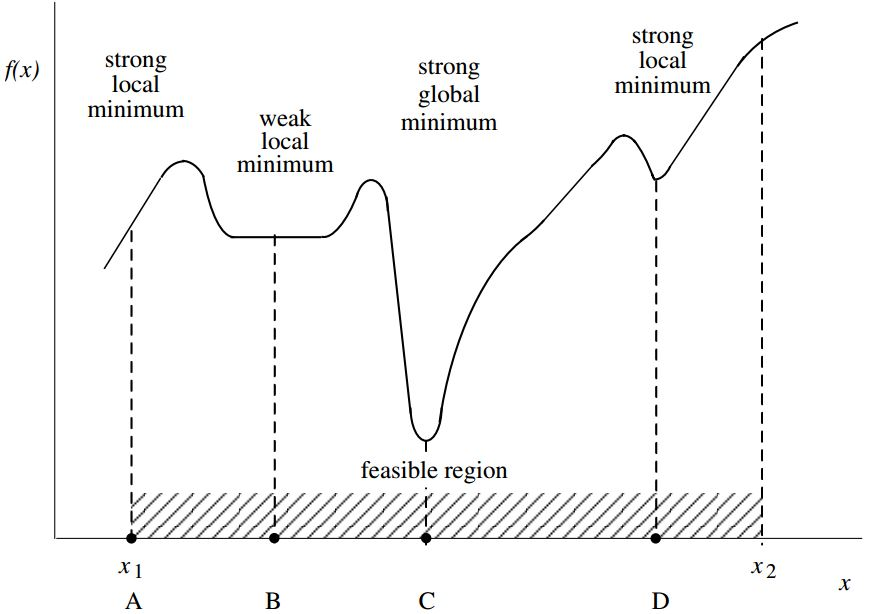
\includegraphics[width=\linewidth]{Images/min.jpg}
	\caption{Minimization points plotted}
\end{figure}
$\tilde{x}=x+\delta \quad \delta =\tilde{x}-x$ $\hat{f}(\tilde{x})=f(x)+g(x)(\tilde{x}-x)^T+0.5(\tilde{x}-x)^T H(x)(\tilde{x}-x)^T$
The gradient $g(x)$ and the Hessian $H(x)$ must satisfy certain conditions at a
local minimizer $x^*$.  \newline
1. Conditions which are satisfied at a local minimizer $x^*$.  \newline
2. Conditions which guarantee that $x^*$ is a local minimizer. 

\textbf{Definition 2.1} A point $x^* \in R,$ where R is the feasible region, is said to be a
weak local minimizer of f(x) if there exists a distance $\epsilon > 0$ such that
$f(x) \geq f(x^*)$ (2.5)
if
$x \in R$ and 
$||x-x^*|| < \epsilon$ \newline

\textbf{Definition 2.2} 
A point $x^* \in R $ is said to be a weak global minimizer of f(x) if
$f(x) \geq f(x^*)$ (2.6)
for all $x \in R.$  \newline
\textbf{Definition 2.3} 

If Eq. (2.5) in Def. 2.1 or Eq. (2.6) in Def. 2.2 is replaced by
$f(x) > f(x^*)$ (2.7)
$x^*$ is said to be a strong local (or global) minimizer. d

\textbf{Definition 2.4} Let $\delta = \alpha \mathbf{d}$ be a change in x where $\alpha$ is a positive constant and d is a direction vector. If R is the feasible region and a constant $\hat{\alpha} > 0$ exists such that
$x + \alpha d \in R$ for all $\alpha$ in the range $0 \leq \alpha \leq \hat{\alpha}$ , then d is said to be a feasible direction at
point x. \newline 

\textbf{Definition 2.5} \newline
(a) Let $d$ be an arbitrary direction vector at point $x$. The quadratic form
$d^TH(x)d$ is said to be \textit{positive definite, positive semidefinite, negative
	semidefinite, negative definite} if $d^TH(x)d > 0, \geq 0, \leq 0, < 0,$ respectively, for all $d \neq 0$ at $x$. If $d^TH(x)d$ can assume positive as well
as negative values, it is said to be indefinite. \newline
(b) If $d^TH(x)d$ is positive definite, positive semidefinite, etc., then matrix
$H(x)$ is said to be positive definite, positive semidefinite, etc. \newline

The objective function must satisfy two sets of conditions in order to have
a minimum, namely, first- and second-order conditions.  \newline
\textbf{First-order necessary conditions for a minimum} \newline %Theorem 2.2
(a) If $f(x) \in C^1$ and $x^*$ is a local minimizer, then
$g(x^*)^Td \geq 0$ for every feasible direction $d$ at $x^*$. \newline
(b) If $x^*$ is located in the interior of $\mathcal{R}$ then
$g(x^*) = 0$ \newline \newline 
\textbf{Second-order necessary conditions for a minimum} \newline
%Theorem 2.2
(a) If $f(x) \in C_2$ and $x^*$ is a local minimizer, then for every feasible direction
d at $x^*$. \hfill \break
\indent     $(i) \ g(x^*)Td \geq 0$ \newline
\indent    $(ii)$ If $g(x^*)^Td = 0$, then $d^TH(x^*)d \geq 0$ \newline
(b) If $x^*$ is a local minimizer in the interior of R, then \newline
\indent $ (i)$ $g(x^*) = 0$ \newline
\indent $ (ii)$ $d^TH(x^*)d \geq 0$ for all $d \neq 0$ 

\textbf{Second-order sufficient conditions for a minimum} \newline %Theorem 2.5
If $f(x) \in C_2$
and $x^*$ is located in the interior of $\mathcal{R}$, then the conditions
(a) $g(x^*) = 0$
(b) $H(x^*)$ is positive definite
are sufficient for $x^*$ to be a strong local minimizer. \newline

\textbf{Definition 2.6} \newline
A point $\bar{x} \in \mathcal{R},$ where $\mathcal{R}$ is the feasible region, is said to be a saddle point if \newline
(a) $g(\bar{x}) = 0$ \newline
(b) point $\bar{x}$ is neither a maximizer nor a minimizer. \hfill \break \newline
Stationary points can be located and classified as follows: \newline
1. Find the points $x_i$ at which $g(x_i) = 0$. \newline
2. Obtain the Hessian $H(x_i)$. \newline
3. Determine the character of $H(x_i)$ for each point $x_i$. \newline
If $H(x_i)$ is positive (or negative) definite, $x_i$ is a minimizer (or maximizer);
if $H(x_i)$ is indefinite, $x_i$ is a saddle point. 

\textbf{Techniques to compute Hessian P.D. , N.D. } \newline
Eigenvalues: det $ (\lambda I -A) = 0$ Multiplying all eigenvalues is equal to the determinant. \newline
The leading principal minors of a matrix A or its negative $-A$ can be used to
establish whether the matrix is positive or negative definite whereas the principal
minors of A or $-A$ can be used to establish whether the matrix is positive or
negative semidefinite. \newline 

\textbf{Theorem 2.9 Properties of matrices} \newline 
(a) If \textbf{H} is positive semidefinite or positive definite, then
det $\mathbf{H} \geq 0  \ \text{or} > 0$ \newline 
(b) \textbf{H} is positive definite if and only if all its leading principal minors are
positive, i.e., det $\mathbf{H_i} > 0$ for $ i = 1, 2, \cdots , n.$ \newline 
(c) \textbf{H} is positive semidefinite if and only if all its principal minors are nonnegative, i.e., det $(H_i^{(l)}) \geq 0$ for all possible selections of $\{l_1, l_2, \cdots , l_i \}$
for $i = 1, 2, \cdots, n$. \newline 
(d) \textbf{H} is negative definite if and only if all the leading principal minors of
$-\mathbf{H}$ are positive, i.e., $det ( -H_i) > 0$ for $i = 1, 2, \cdots, n$. \newline 
(e) \textbf{H} is negative semidefinite if and only if all the principal minors of -$\mathbf{H}$
are nonnegative, i.e., det $(-H_i^{(l)}) \geq 0$ for all possible selections of
$\{l_1, l_2, \cdots , l_i \}$ for $i = 1, 2, \cdots , n$. \newline 
(f) \textbf{H} is indefinite if neither (c) nor (e) holds. 

\textbf{Definition 2.7} \newline
A set $\mathcal{R}_c
\subset E_n $ is said to be convex if for every pair of points $x_1, x_2 \subset R_c$
and for every real number $\alpha$ in the range $0 < \alpha < 1$, the point
$x = \alpha x_1 + (1 - \alpha)x_2$
is located in $\mathcal{R}_c
$, i.e., $x \in \mathcal{R}_c$. \newline 

\textbf{Definition 2.8} \newline
(a) A function $f(x)$ defined over a convex set $\mathcal{R}_c$  is said to be convex if for
every pair of points $x_1, x_2 \in \mathcal{R}_c $ and every real number $\alpha$ in the range $0 < \alpha < 1$, the inequality
$f[\alpha x_1 + (1 - \alpha)x_2] \leq \alpha f(x_1) + (1 - \alpha)f(x_2)$ 
holds. If $x_1 \neq x_2$ and
$f[\alpha x_1 + (1 - \alpha)x_2] < \alpha f(x_1) + (1 - \alpha)f(x_2)$
then f(x) is said to be strictly convex. \newline
(b) If $\phi(x)$ is defined over a convex set $\mathcal{R}_c$ and f(x) = -$\phi(x)$ is convex, then $\phi(x)$ is said to be concave. If f(x) is strictly convex, $\phi(x)$ is strictly concave. \newline

\textbf{Property of convex functions relating to the Hessian} A function $f(x) \in C^2$is convex over a convex set 
$\mathcal{R}_c$ if and only if the Hessian H(x) of
f(x) is positive semidefinite for $x \in \mathcal{R}_c.$  \newline 

\textbf{Theorem 2.15 Relation between local and global minimizers in convex functions} \newline 
If $f(x)$ is a convex function defined on a convex set $\mathcal{R}_c$, then  \newline 
(a) the set of points $S_c$ where $f(x)$ is minimum is convex;  \newline 
(b) any local minimizer of $f(x)$ is a global minimizer. 

\section{Ch. 4}
\textbf{Dichotomous Search} \newline
Two function evaluations per iteration. \newline
A \textbf{unimodal function} on an interval has exactly
one point where a maximum or minimum
occurs in the interval. \newline 
Consider a unimodal function which is known to have a minimum in the interval $[x_L, \ x_U]$. This interval is said to be the range of uncertainty. \newline 
In this method, f(x) is evaluated at two points $x_a =
x_1 - \epsilon/2$ and $x_b = x_1 +\epsilon/2$ where $\epsilon$ is a small positive number. Then depending
on whether $f(x_a) < f(x_b)$ or $f(x_a) > f(x_b)$, range $x_L$ to $x_1 + \epsilon/2$ or $x_1 - \epsilon/2$
to $x_U$ can be selected and if $f(x_a) = f(x_b)$ either will do fine. If we assume
that $x_1 - x_L = x_U - x_1$, i.e., $x_1 = (x_L + x_U)/2$, the region of uncertainty
is immediately reduced by half. The same procedure can be repeated for the
reduced range, that is, f(x) can be evaluated at $x_2 - \epsilon/2$ and $x2 + \epsilon/2$ where $x_2$ is located at the center of the reduced range, and so on. \newline \newline 
%\begin{Figure}
%	\centering
%	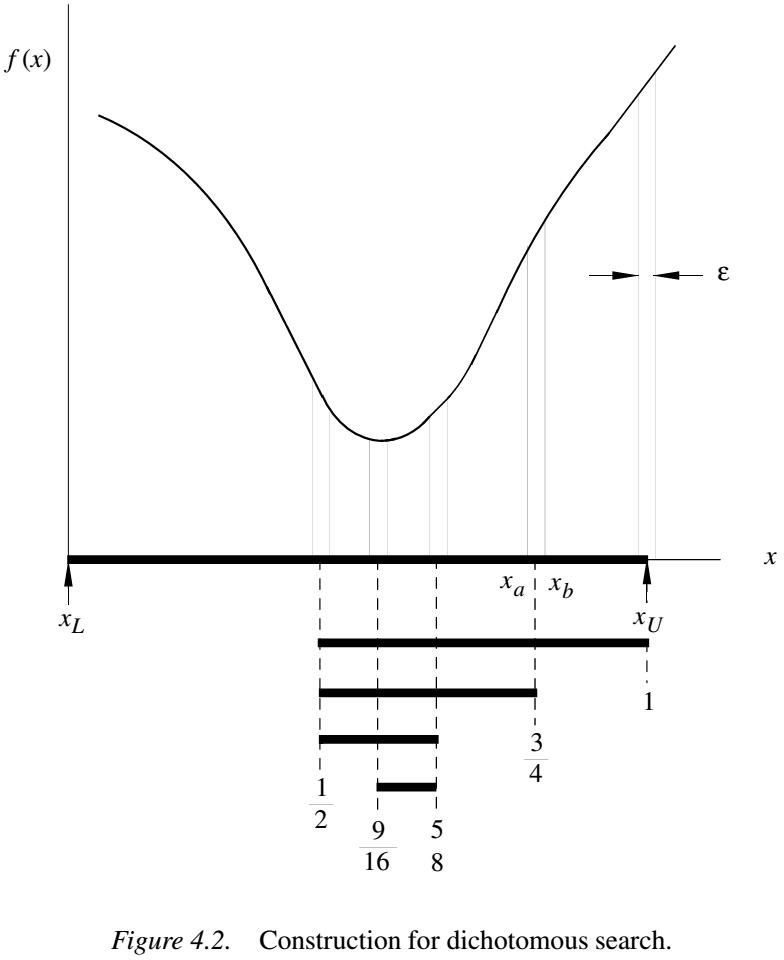
\includegraphics[width=\linewidth]{disearch}
%\end{Figure}
\textbf{Algorithm 4.1 Fibonacci} \newline
Computing n =$I_n=\frac{I_1}{F_n}$, function evaluations = n-1 \newline
\textbf{Step 1} \newline
Input $x_{L,1}, x_{U,1}$, and n. \newline
\textbf{Step 2} \newline
Compute $F_1, F_2, \cdots, F_n$ using Eq. (4.4). \newline
\textbf{Step 3} \newline
Assign $I_1 = x_{U,1} - x_{L,1}$ and compute
\begin{align*}
& I_2 = \frac{F_{n -1}}{F_n}I_1 (\text{see Eq. (4.6)})\\
& x_{a,1} = x_{U,1} - I_2, \quad x_{b,1} = x_{L,1} + I_2\\ 
& f_{a,1} = f(x_{a,1}), \quad f_{b,1} = f(x_{b,1})
\end{align*}
Set k = 1. \newline
\textbf{Step 4} \newline
Compute $I_{k+2}$ using Eq. (4.6).
If $f_{a,k} \geq f_{b,k}$, then update Eqs. (4.7) to (4.12) using
\begin{align*}
& x_{L,k+1}=x_{a,k} \\
& x_{U,k+1}=x_{U,k} \\
& x_{a,k+1}=x_{b,k} \\
& x_{b,k+1}=x_{L,k+1}+I_{k+1} \\
& f_{a,k+1}=f_{b,k} \\
& f_{b,k+1}=f(x_{b,k+1})
\end{align*}
using  Otherwise, if $f_{a,k} < f_{b,k}$, update
information using Eqs. (4.13) to (4.18) using \newline
\begin{align*}
& x_{L,k+1}=x_{L,k} \\
& x_{U,k+1}=x_{b,k} \\
& x_{a,k+1}=x_{U,k+1}-I_{k+2} \\
& x_{b,k+1}=x_{a,k} \\
& f_{a,k+1}=f(x_{a,k+1}) \\
& f_{b,k+1}=f_{a,k}
\end{align*}

\textbf{Step 5} \newline
If $k = n - 2$ or $x_{a,k+1} > x_{b,k+1}$, output $x^* = x_{a,k+1}$ and $f^* = f(x^*)$,
and stop. Otherwise, set $k = k + 1$ and repeat from Step 4.
The condition $x_{a,k+1} > x_{b,k+1}$ implies that $x_{a,k+1} \approx x_{b,k+1}$ within the precision of the computer used, as was stated earlier, or that there is an error in the algorithm. It is thus used as an alternative stopping criterion. \newline

\textbf{Algorithm 4.2 Golden-section search} \newline
(function evaluations = k+1) and Golden Ratio: $K=\cfrac{1+\sqrt{5}}{2}$
$\Lambda_{GS} = I_n = \frac{I_1}
{K_{n-1}}$ \quad $\Lambda_{F} = I_n = \frac{I_1}
{F_n} \approx \frac{\sqrt{5}}
{K^{n+1}}I_1$
$\frac{I_k}{I_{k+1}}=\frac{I_{k+1}}{I_{k+2}}
= \frac{I_{k+2}}{I_{k+3}}
= \cdots = K$ \newline
\textbf{Step 1} \newline
Input $x_{L,1}, x_{U,1},$ and $\epsilon$. \newline
\textbf{Step 2} \newline
Assign $I_1 = x_{U,1} - x_{L,1}, K = 1.618034$ and compute
\begin{align*}
&I_2 = I_1/K \\
&x_{a,1} = x_{U,1} - I_2, \quad x_{b,1} = x_{L,1} + I_2 \\
&f_{a,1} = f(x_{a,1}), \quad f_{b,1} = f(x_{b,1}) 
\end{align*}
Set $k = 1$. \newline
\textbf{Step 3} \newline
Compute $I_{k+2} = I_{k+1}/K$ \newline
If $f_{a,k} \geq f_{b,k}$, then update $x_{L,k+1}, x_{U,k+1}$, $x_{a,k+1}$, $x_{b,k+1}$, $f_{a,k+1}$,
and $f_{b,k+1}$ as  
\begin{align*}
& x_{L,k+1}=x_{a,k} \\
& x_{U,k+1}=x_{U,k} \\
& x_{a,k+1}=x_{b,k} \\
& x_{b,k+1}=x_{L,k+1}+I_{k+1} \\
& f_{a,k+1}=f_{b,k} \\
& f_{b,k+1}=f(x_{b,k+1})
\end{align*}
Or use using Eqs. (4.7) to (4.12). 
Otherwise if $f_{a,k} < f_{b,k}$, then update $x_{L,k+1}, x_{U,k+1}$, $x_{a,k+1}$, $x_{b,k+1}$, $f_{a,k+1}$, and $f_{b,k+1}$ as
\begin{align*}
& x_{L,k+1}=x_{L,k} \\
& x_{U,k+1}=x_{b,k} \\
& x_{a,k+1}=x_{U,k+1}-I_{k+2} \\
& x_{b,k+1}=x_{a,k} \\
& f_{a,k+1}=f(x_{a,k+1}) \\
& f_{b,k+1}=f_{a,k}
\end{align*}
Otherwise, if $f_{a,k} < f_{b,k}$, update
information using Eqs. (4.13) to (4.18). \newline
\textbf{Step 4} \newline
If $I_k < \epsilon$ or $x_{a,k+1} > x_{b,k+1}$, then do: \newline
If $f_{a,k+1} > f_{b,k+1}$, compute
$x^* = 0.5(x_{b,k+1} + x_{U,k+1})$ \newline
If $f_{a,k+1} = f_{b,k+1}$, compute
$x^* = 0.5(x_{a,k+1} + x_{b,k+1})$ \newline
If $f_{a,k+1} < f_{b,k+1}$, compute
$x^* = 0.5(x_{L,k+1} + x_{a,k+1})$
Compute $f^* = f(x^*).$ \newline
Output $x^*$ and $f^*$, and stop. \newline
\textbf{Step 5} \newline
Set $k = k + 1$ and repeat from Step 3. \newline \newline 
\textbf{Equations 4.4, 4.6, (4.7-4.12) and (4.13-4.18) } \newline
$F_k = F_{k-1} + F_{k-2} \quad$ for $k \geq 2$ (4.4) \newline
$I_{k+2} = \frac{F_{n-k-1}}{F_{n-k}}I_{k+1} (4.6)$

If $f_{a,k} > f_{b,k}$, then $x^*$ is in interval $[x_{a,k}, x_{U,k}]$ and so the new bounds of $x^* \rightarrow$  %\newline 
$x_{L,k+1} = x_{a,k} (4.7) \quad x_{U,k+1} = x_{U,k} (4.8)$ 
Similarly, the two interior points of the new interval, namely, $x_{a,k+1}$ and $x_{b,k+1}$
will be $x_{b,k}$ and $x_{L,k+1} + I_{k+2}$, respectively. We can thus assign
$x_{a,k+1} = x_{b,k}$ (4.9) $x_{b,k+1} = x_{L,k+1} + I_{k+2}$ (4.10)
as illustrated in Fig. 4.5. \newline
The value $f_{b,k}$ is retained as the value of f(x) at
$x_{a,k+1}$, and the value of f(x) at $x_{b,k+1}$ is calculated, i.e.,
$f_{a,k+1} = f_{b,k}$ (4.11)
$f_{b,k+1} = f(x_{b,k+1})$ (4.12) \newline
%\begin{Figure}
%	\centering
%	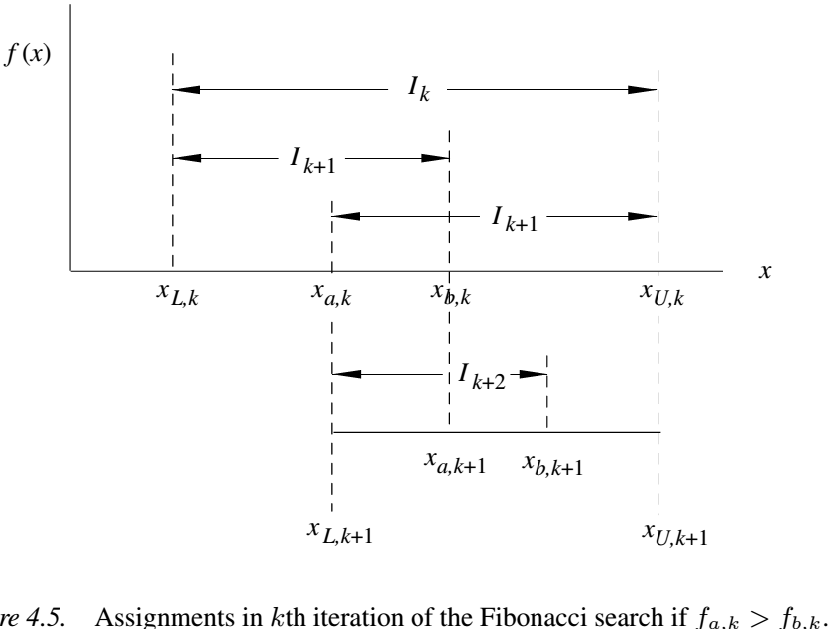
\includegraphics[width=\linewidth]{fibfirst}
%\end{Figure}
On the other hand, if $f_{a,k} < f_{b,k}$, then $x^*$ is in interval $[x_{L,k}, x_{b,k}]$. In this
case, we assign
$x_{L,k+1} = x_{L,k}$ (4.13)
$x_{U,k+1} = x_{b,k}$ (4.14)
$x_{a,k+1} = x_{U,k+1} - I_{k+2}$ (4.15)
$x_{b,k+1} = x_{a,k}$ (4.16)
$f_{b,k+1} = f_{a,k}$ (4.17)
and calculate
$f_{a,k+1} = f(x_{a,k+1})$ (4.18) \newline  \newline
%\begin{Figure}
%	\centering
%	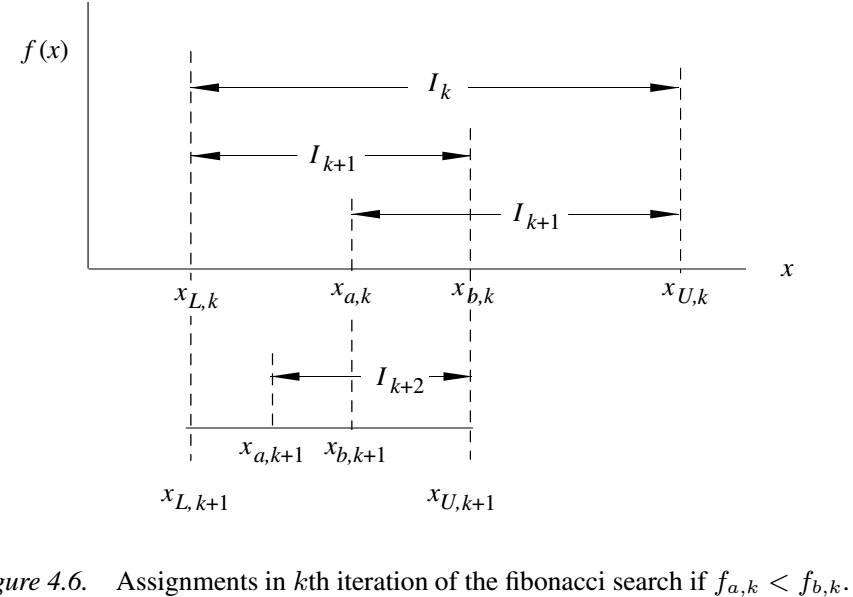
\includegraphics[width=\linewidth]{fibsecond}
%\end{Figure}
%\begin{Figure}
%	\centering
%	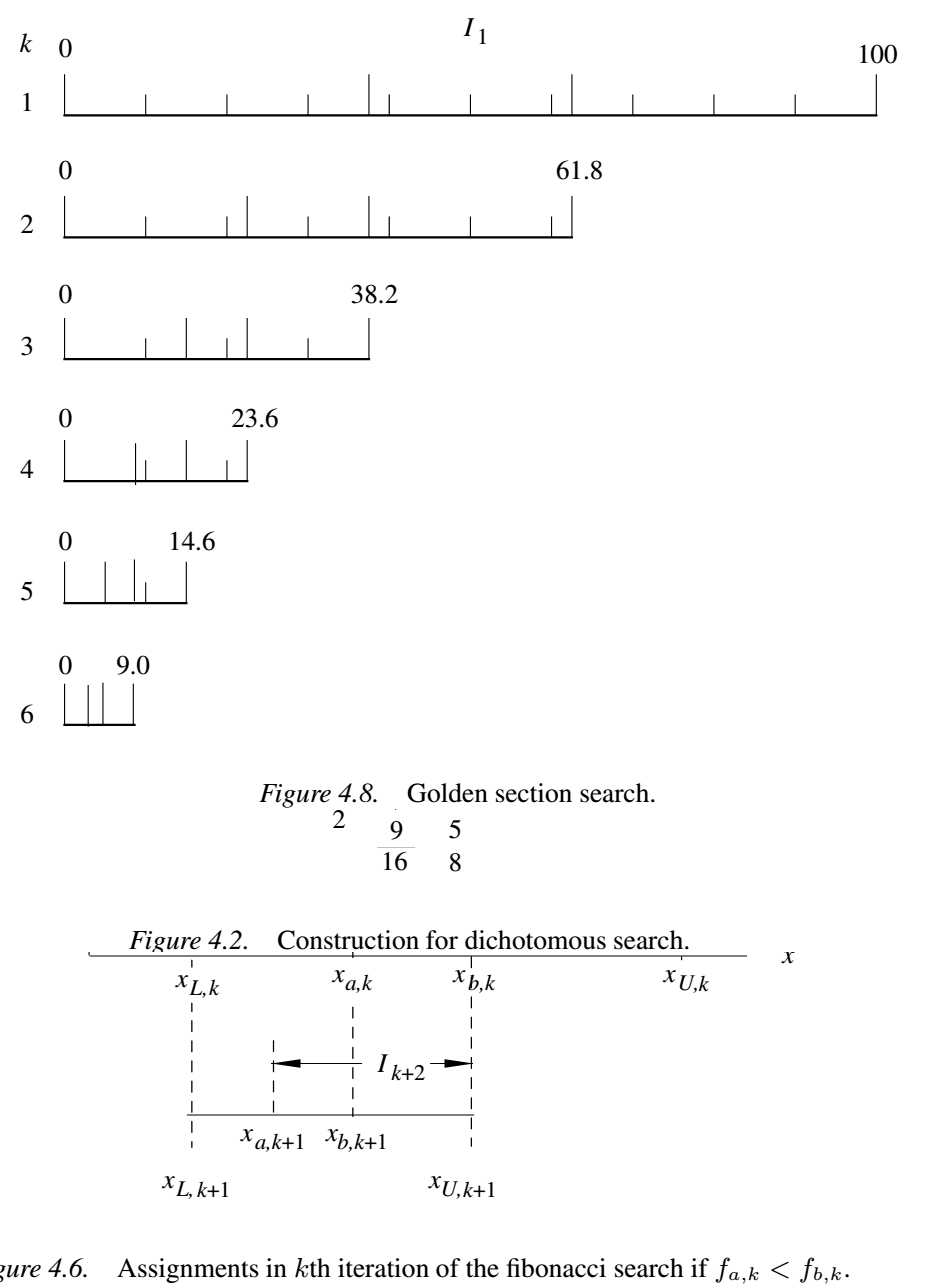
\includegraphics[width=\linewidth]{golden}
%\end{Figure}
%\begin{Figure}
%	\centering
%	\includegraphics[width=\linewidth]{fib}
%\end{Figure}
%%%%%%%%%%%%%%%%%%%%%%%%%%%%%%%
%% Unlikely to be tested %%
%% INCLUDE FOR FINAL %%
%%%%%%%%%%%%%%%%%%%%%%%%%%%%%%%
\textbf{Algorithm 4.6 Inexact line search}  \newline
\textbf{Step 1:} \newline
Input $x_k$, $d_k$, and compute $g_k$. \newline
Initialize algorithm parameters $\rho, \sigma, \tau$, and $\chi$. \newline
Set $\alpha_L = 0$ and $\alpha_U = 10^{99}$. \newline
\textbf{Step 2:} \newline
Compute $f_L = f(x_k + \alpha_L dk)$. \newline
Compute $f_L^\prime = g(x_k + \alpha_L dk)^Tdk$. \newline
\textbf{Step 3:} \newline
Estimate $\alpha_0$. \newline
\textbf{Step 4:} \newline
Compute $f_0 = f(x_k + \alpha_0dk)$. \newline
\textbf{Step 5 (Interpolation)} \newline
If $f_0 > f_L + \rho(\alpha_0 - \alpha_L)f_L^\prime$ , then do: \newline
a. If $\alpha_0 < \alpha_U$, then set $\alpha_U = \alpha_0$.\newline
b. Compute $\breve{\alpha}_0$ using the interpolation formula Eq. (4.57). %\newline
\[
\breve{\alpha}_0 =\alpha_L + \frac{(\alpha_0-\alpha_L)^2f_L^\prime}{2[f_L-f_0+(\alpha_0-\alpha_L)f_L^\prime]}
\]
c. If $\breve{\alpha}_0 < \alpha_L + \tau(\alpha_U - \alpha_L)$ then set $\breve{\alpha}_0 = \alpha_L + \tau(\alpha_U - \alpha_L)$. \newline
d. If $\breve{\alpha}_0 > \alpha_U - \tau(\alpha_U - \alpha_L)$ then set $\breve{\alpha}_0  = \alpha_U - \tau(\alpha_U - \alpha_L)$. \newline
e. Set $\alpha_0 = \breve{\alpha}_0$ and go to Step 4. \newline
\textbf{Step 6} \newline
Compute $f_0^\prime = g(x_k + \alpha_0dk)^Tdk$. \newline
\textbf{Step 7 (Extrapolation)} \newline
If $f_0^\prime < \alpha f_L^\prime$ , then do: \newline
a. Compute $\nabla \alpha_0 = (\alpha_0 - \alpha_L)f_0^\prime /(f_L^\prime - f_0^\prime)$ (see Eq. (4.58)).
\[
\breve{\alpha}_0 = \alpha_0 + (\alpha_0 - \alpha_L)f_0^\prime
(f_L^\prime - f_0^\prime) \quad (Eq. (4.58))
\]
b. If $\nabla \alpha_0 < \tau(\alpha_0 - \alpha_L)$, then set $\nabla \alpha_0 = \tau(\alpha_0 - \alpha_L)$. \newline
c. If $\nabla \alpha_0 > \chi(\alpha_0 - \alpha_L)$, then set $\nabla \alpha_0 = \chi(\alpha_0 - \alpha_L)$. \newline
d. Compute $\breve{\alpha}_0 = \alpha_0 + \nabla \alpha_0$. \newline
e. Set $ \alpha_L =  \alpha_0, \alpha_0 = \breve{\alpha}_0, f_L = f_0, f_L^\prime = f_0^\prime$, and go to Step 4. \newline
\textbf{Step 8} \newline
Output $\alpha_0$ and $f_0 = f(x_k + \alpha_0dk)$, and stop.


\section{Ch. 5}
Standard form: $f(x)=\frac{1}{2}x^T H x + x^T g(x) + C$ \newline 
Rate of Convergence $\beta = (1-r^2)/(1+r^2)$, where r is the smallest eigenvalue divided by the biggest eigenvalue. \newline
\begin{align*}
& H^{-1}=\begin{bmatrix}
a & c \\
c & b 
\end{bmatrix}^{-1}
=
\frac{1}{ab-c^2}
\begin{bmatrix}
b & -c \\
-c & a
\end{bmatrix} \quad ab-c^2 \neq 0
\end{align*}
$[f(x_k)-f(x^*)]\leq \left(\frac{1-r}{1+r}\right)^2[f(x_k)-f(x^*)]$ \newline
\textbf{Algorithm 5.1 Steepest-descent algorithm} \newline
\textbf{Step 1}  \newline
Input $x_0$ and initialize the tolerance $\epsilon$. \newline
Set $k = 0$. \newline
\textbf{Step 2} \newline
Calculate gradient $g_k$ and set $d_k=-g_k$. \newline
\textbf{Step 3} \newline
Find $\alpha_k$, the value of $\alpha$ that minimizes $f(x_k + \alpha d_k)$, using a line search (Algorithm Inexact Line Search. 4.6). \newline
\textbf{Step 4} \newline
Set $x_{k+1} = x_k + \alpha_k d_k$ and calculate $f_{k+1} = f(x_{k+1})$. \newline
\textbf{Step 5}  \newline
If $||\alpha_k d_k|| < \epsilon$, then do: \newline
Output $x^* = x_{k+1}$ and $f(x^*) = f_{k+1}$, and stop. \newline
Otherwise, set $k = k + 1$ and repeat from Step 2. \newline 

\textbf{Algorithm 5.3 Basic Newton algorithm} \newline
\textbf{Step 1} \newline
Input $x_0$ and initialize the tolerance $\epsilon$ \newline
Set $k = 0$. \newline
\textbf{Step 2} \newline
Compute $g_k$ and $H_k$. \newline
If $H_k$ is not positive definite, force it to become positive definite. \newline
\textbf{Step 3} \newline
Compute $H_k^{-1}$ and $d_k=-H_k^{-1}g_k$ \newline
\textbf{Step 4} \newline
Find $\alpha_k$ , the value of $\alpha$ that minimizes $f(x+\alpha d_k)$, using a line search. \newline
\textbf{Step 5} \newline
Set $x_{k+1}=x_k+\alpha_k d_k$ \newline
Compute $f_{k+1}=f(x_{k+1})$. \newline
\textbf{Step 6} \newline
If $||\alpha_k d_k|| < \epsilon$, then do:  \newline
Output $x^*=x_{k+1}$ and $f(x^*)=f(x_{k+1})$, and stop \newline
Otherwise, set $k = k + 1$ and repeat from Step 2. \newline
\textbf{Algorithm 5.5 Gauss --- Newton Algorithm} \newline
$f=\begin{bmatrix}
f_1(x)  & f_2(x) & \cdots f_m(x)
\end{bmatrix}^T$, J = Jacobian \newline
$F(x)=\sum_{p=1}^{m}f_p(x)^2=f^Tf$ \newline
$J=\begin{bmatrix}
\frac{ \partial f_1}{\partial  x_1} & \frac{ \partial  f_1}{ \partial  x_2} & \cdots & \frac{\partial  f_1}{\partial  x_n} \\
\frac{\partial  f_2}{\partial x_1} & \frac{\partial  f_2}{\partial  x_2} & \cdots & \frac{\partial  f_2}{\partial x_n} \\
\vdots & \vdots & \ddots & \vdots \\
\frac{\partial f_m}{\partial  x_1}& \frac{\partial f_m}{\partial  x_2}& \cdots & \frac{\partial f_m}{\partial x_n}
\end{bmatrix}$ \newline
\textbf{Step 1} \newline
Input $x_0$ and initialize the tolerance $\epsilon$.  \newline
Set $k = 0$. \newline
\textbf{Step 2} \newline
Compute $f_{pk} = f_p(x_k)$ for $p = 1, 2, \cdots, m$ and $F_k$.
\newline
\textbf{Step 3}  \newline
Compute $J_k, g_k = 2J^T_k f_k$, and $H_k = 2J^T_k J_k$. \newline
\textbf{Step 4}  \newline
$d_k=-H_k^{-1}g_k$ \newline
\textbf{Step 5} \newline
Find $\alpha_k$, the value of $\alpha$ that minimizes $f(x_k + \alpha d_k)$. \newline
\textbf{Step 6} \newline
Set $x_{k+1} = x_k + \alpha_kd_k$. \newline
Compute $f_{p,k+1}$ for $p = 1, 2,\cdots, m$ and $F_{k+1}$. \newline
\textbf{Step 7} \newline
If $|F_{k+1}-F_k | < \epsilon$, then do: \newline
Output $x^*= x_{k+1}$, $f_{p,k+1}(x^*)$ for $p = 1, 2,\cdots, m$, and $F_{k+1}$. \newline
Stop. \newline
Otherwise, set $k = k + 1$ and repeat from Step 3.


\section{Ch. 7}
\textbf{Problems with Rank-one Method}
\begin{enumerate}
	\item positive definite $S_k$ may not yield positive definite $S_{k+1}$
	\item denominator in correction formula may approach zero 
\end{enumerate}  
THE DFP and BFGS are implementing of the basic algorithms Quasi Newton (7.2) with changes to the updating function. $d_k=-S_kg_k$ and $f(x_k + \alpha d_k)$  $\rightarrow$  $\alpha_k=\frac{g_k^TS_kg_k} 
{g_k^TS_kHS_kg_k}$ \newline
Convergence equation: $\beta = \left(\frac{1-r}{1+r}\right)^2$ $f(x_{k+1})-f(x^*) \leq \left(\frac{1-r}{1+r}\right)^2[f(x_k)-f(x^*)]$ \newline
\textbf{BFGS and then DFP properties} \newline
For convex quadratic functions (BFGS)
\begin{enumerate}
	\item[---] $Sk+1$ becomes identical to $H^{-1}$ for $k = n-1$.
	\item[---] Directions $\delta_0,\delta_1,\cdots,\delta_{n-1}$ form a conjugate set. 
	\item[---] $S_{k+1}$ is positive definite if $S_k$ is positive definite.
	\item[---] $\delta^T_k \gamma_k = \delta^T_k g_{k+1}-\delta_T^k g_k > 0$ applies. \newline
\end{enumerate}  
\textbf{For DFP (from textbook)} 
\begin{enumerate}
	\item If $S_k$ is PD, then 
	the matrix $S_{k+1}$ generated by DFP is also PD.
	\item Directions $\delta_0,\delta_1,\cdots,\delta_{n-1}$ form a conjugate set. \newline
\end{enumerate} 
\textbf{Algorithm 7.2 adjusted for DFP/BFGS} \newline
\textbf{Step 1} \newline
Input $x_0$  and initialize the tolerance $\epsilon$. \newline
Set $k = 0$ and $S_0 = I_n$. \newline
Compute $g_0$. \newline
\textbf{Step 2} \newline
Set $d_k=-S_kg_k$ \newline
Find $\alpha_k$, the value of $\alpha$ that minimizes $f(x_k+\alpha d_k)$, using a line search \newline
Set $\delta_k=\alpha_k d_k$ and $x_{k+1}=x_k+\delta_k$ \newline
\textbf{Step 3} \newline
If $||\delta_k|| < \epsilon$, output $x^* = x_{k+1}$ and $f(x^*) = f(x_{k+1})$, and stop \\
\textbf{Step 4} \newline
Compute $g_{k+1}$ and set $\gamma_k=g_{k+1}-g_k$ \newline
Compute $S_{k+1}$ using appropriate formula.
\begin{align*}
&\text{Basic/ Rank One:} \quad S_{k+1}=S_k+\frac{(\delta_k-S_k \gamma_k)(\delta_k-S_k \gamma_k)^T}{\gamma_k^T(\delta_k-S_k\gamma_k)}\\
&\text{DFP:}\quad S_{k+1}=S_k+\frac{\delta_k \delta_k^T}{\delta_k^T \gamma_k}-\frac{S_k\gamma_k\gamma_k^TS_k}{\gamma_k^TS_k\gamma_k}\\
&\text{BFGS:} \quad S_{k+1}=S_k+\left(1+\frac{\gamma_k^TS_k\gamma_k}{\gamma_k^T\delta_k}\right)\frac{\delta_k\delta_k^T}{\gamma_k^T\delta_k}-\frac{(\delta_k\gamma_k^TS_k+S_k\gamma_k\delta_k^T)}{\gamma_k^T\delta_k}
\end{align*}
Set $k=k+1$ and repeat from Step 2. \newline
\begin{itemize}
	\item[---] remember that $\left(1+\frac{\gamma_k^TS_k\gamma_k}{\gamma_k^T\delta_k}\right)$ is a single number
	\item[---] $\delta_k\delta_k^T$ is a matrix.
	\item[---] Focus on minimization, $\max[f(x)] =-\min[-f(x)]$
	\item[---] Hessian is positive semidefinite for concave functions.
\end{itemize}
\end{multicols}